\section{Time box 2}
\subsection{Time box planning}
Show meeting in week 11.
\subsubsection{Work to be done in this time box}
\begin{itemize}
	\item ARM to FPGA interface
	\begin{itemize}
		\item Mount
		\item Test
	\end{itemize}
	\item PLC module
	\begin{itemize}
		\item Mount x7
		\item Test
	\end{itemize}
	\item Daemon
	\item Power switch
	\begin{itemize}
		\item Block diagram
	\end{itemize}
	\item Module design
\end{itemize}
\paragraph{Description:}
\begin{description}
	\item[ARM to FPGA interface] The connection between the ARM7 CPU and the FPGA board, has to be mounted, tested and debugged.
	\item[PLC module] The powerline module has to be mounted 7 times for all the groups, tested and debugged.
	\item[Daemon] 
	\item[Power switch] Block diagram of the power switch, which shall activate the different modules connected to it (wind-turbine, photo-voltaic cells etc.) and control the current flow.
	\item[Module design]
\end{description}

\subsection{ARM to FPGA interface - Dennis}
The first version of the PCB was hard to solder because of the small pad sizes. A second version of the interface has been made, with increased pad size and increased clearance between the tracks. Also the Chip select connector pin has been more centralized on the PCB to decrease cable length. The hole in the one site of the PCB is needed to avoid removing a connector on the arm-board, the tracks beside this connector have been rerouted to give more space for this connector. 
\begin{figure}[H]
	\begin{centering}
		 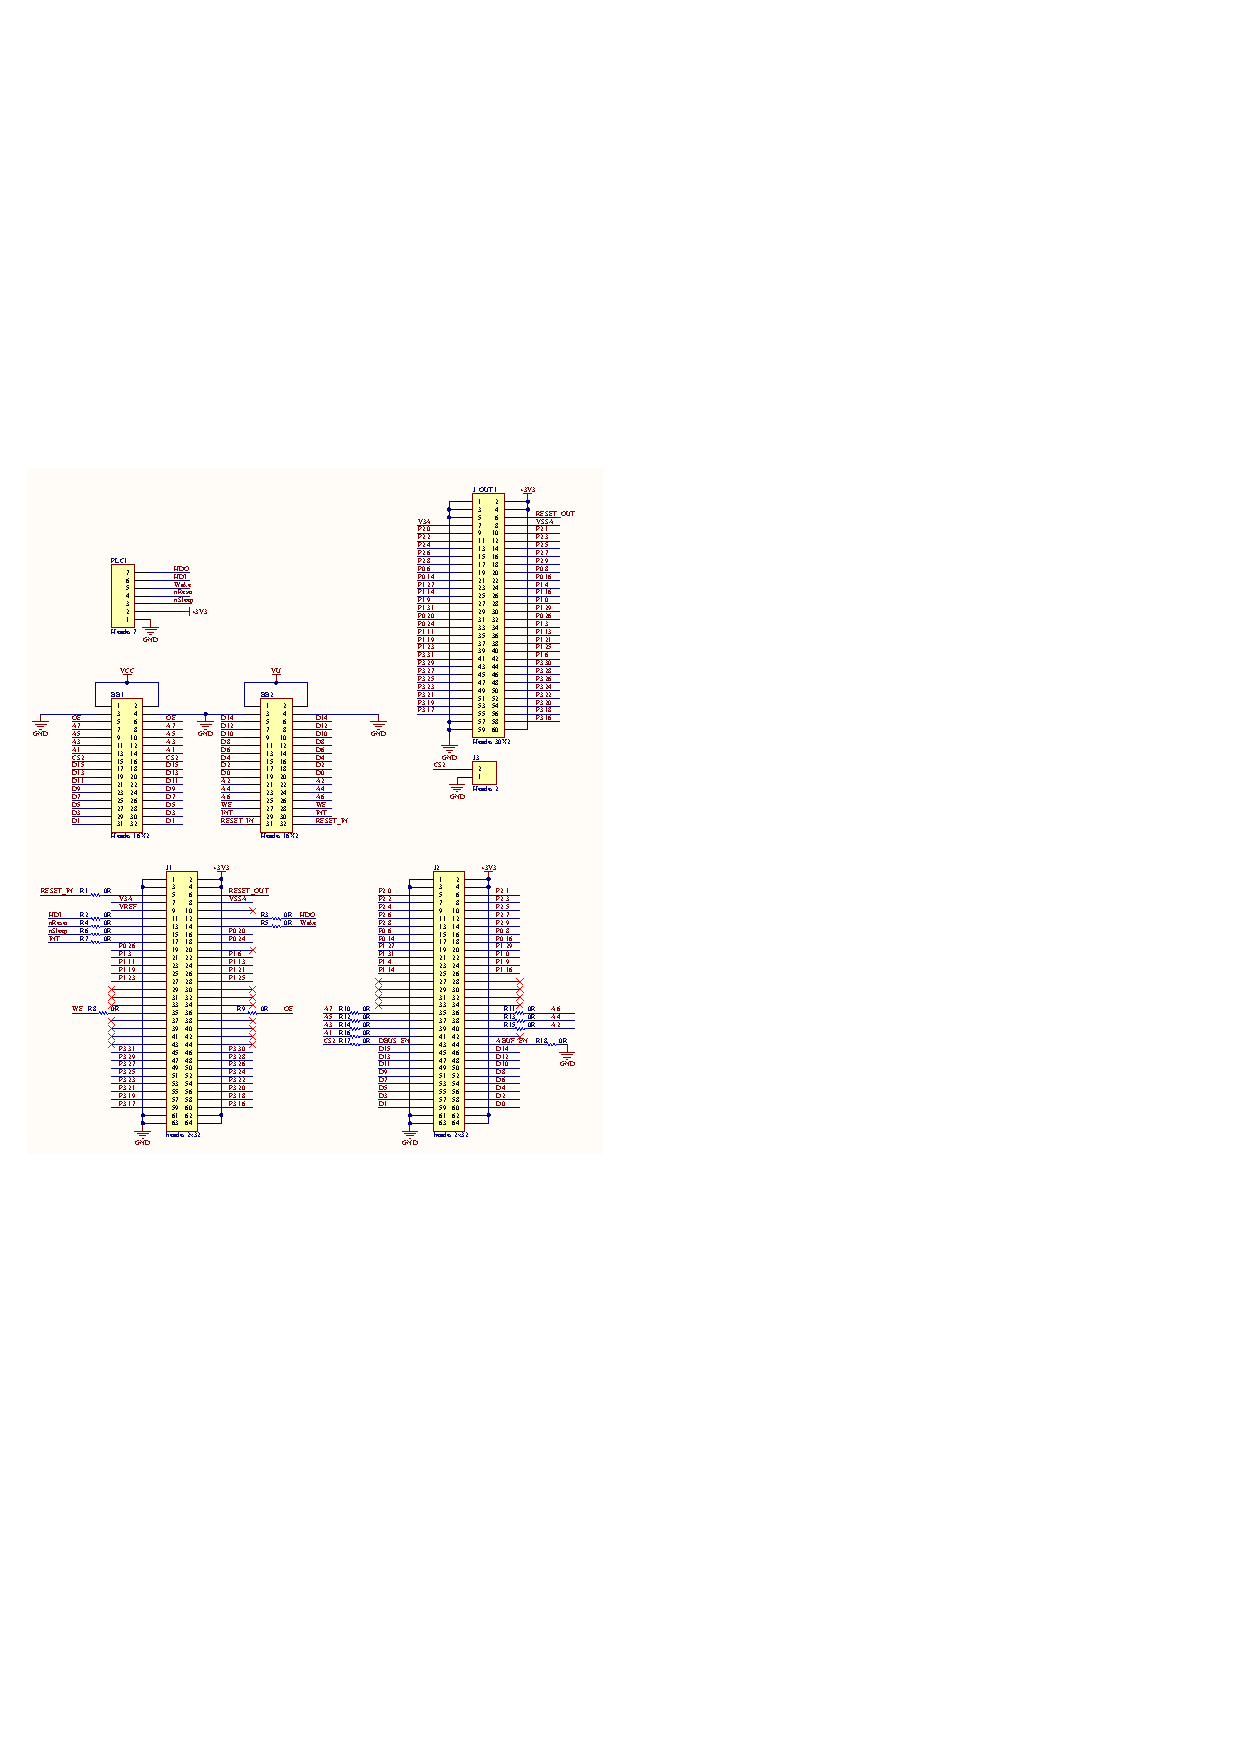
\includegraphics[width=0.60\textwidth,page=1]{images/dig_to_ea_v0_2}
		\caption{Schematic of the ARM to FPGA connector, v0.2.}
	\end{centering}
\end{figure}

\begin{figure}[H]
	\begin{centering}
		 \includegraphics[height=0.8\textwidth,page=2,angle=90]{images/dig_to_ea_v0_2}
		\caption{PCB of the ARM to FPGA connector, v0.2 (top view)}
	\end{centering}
\end{figure}

\todo[inline]{insert picture of soldered and connected connector}

\subsection{PLC module - Dennis}
The second version of the Power line module was decreased in size, which lead to problems when making the PCB, as a lot of tracks short-circuited. A third version with larger clearance between the tracks and the ground plane has been made. The PCB has been mounted and tested, this is describe in the \textit{EPRO 3 \& 4 PLC - Hardware Interface} report. As a short resume, the communication between two boards through power line works without seeing any invalid characters (test period of 15 min.). The 5 volt power supply has been tester to withstand at minimum 2.4 Amp. where a voltage drop of approximately 0.1Volt was observed. 
A single error has been found and corrected before ordering and mounting the 6 PLC boards needed (one for each module in the system/group).

\begin{figure}[H]
	\begin{centering}
		 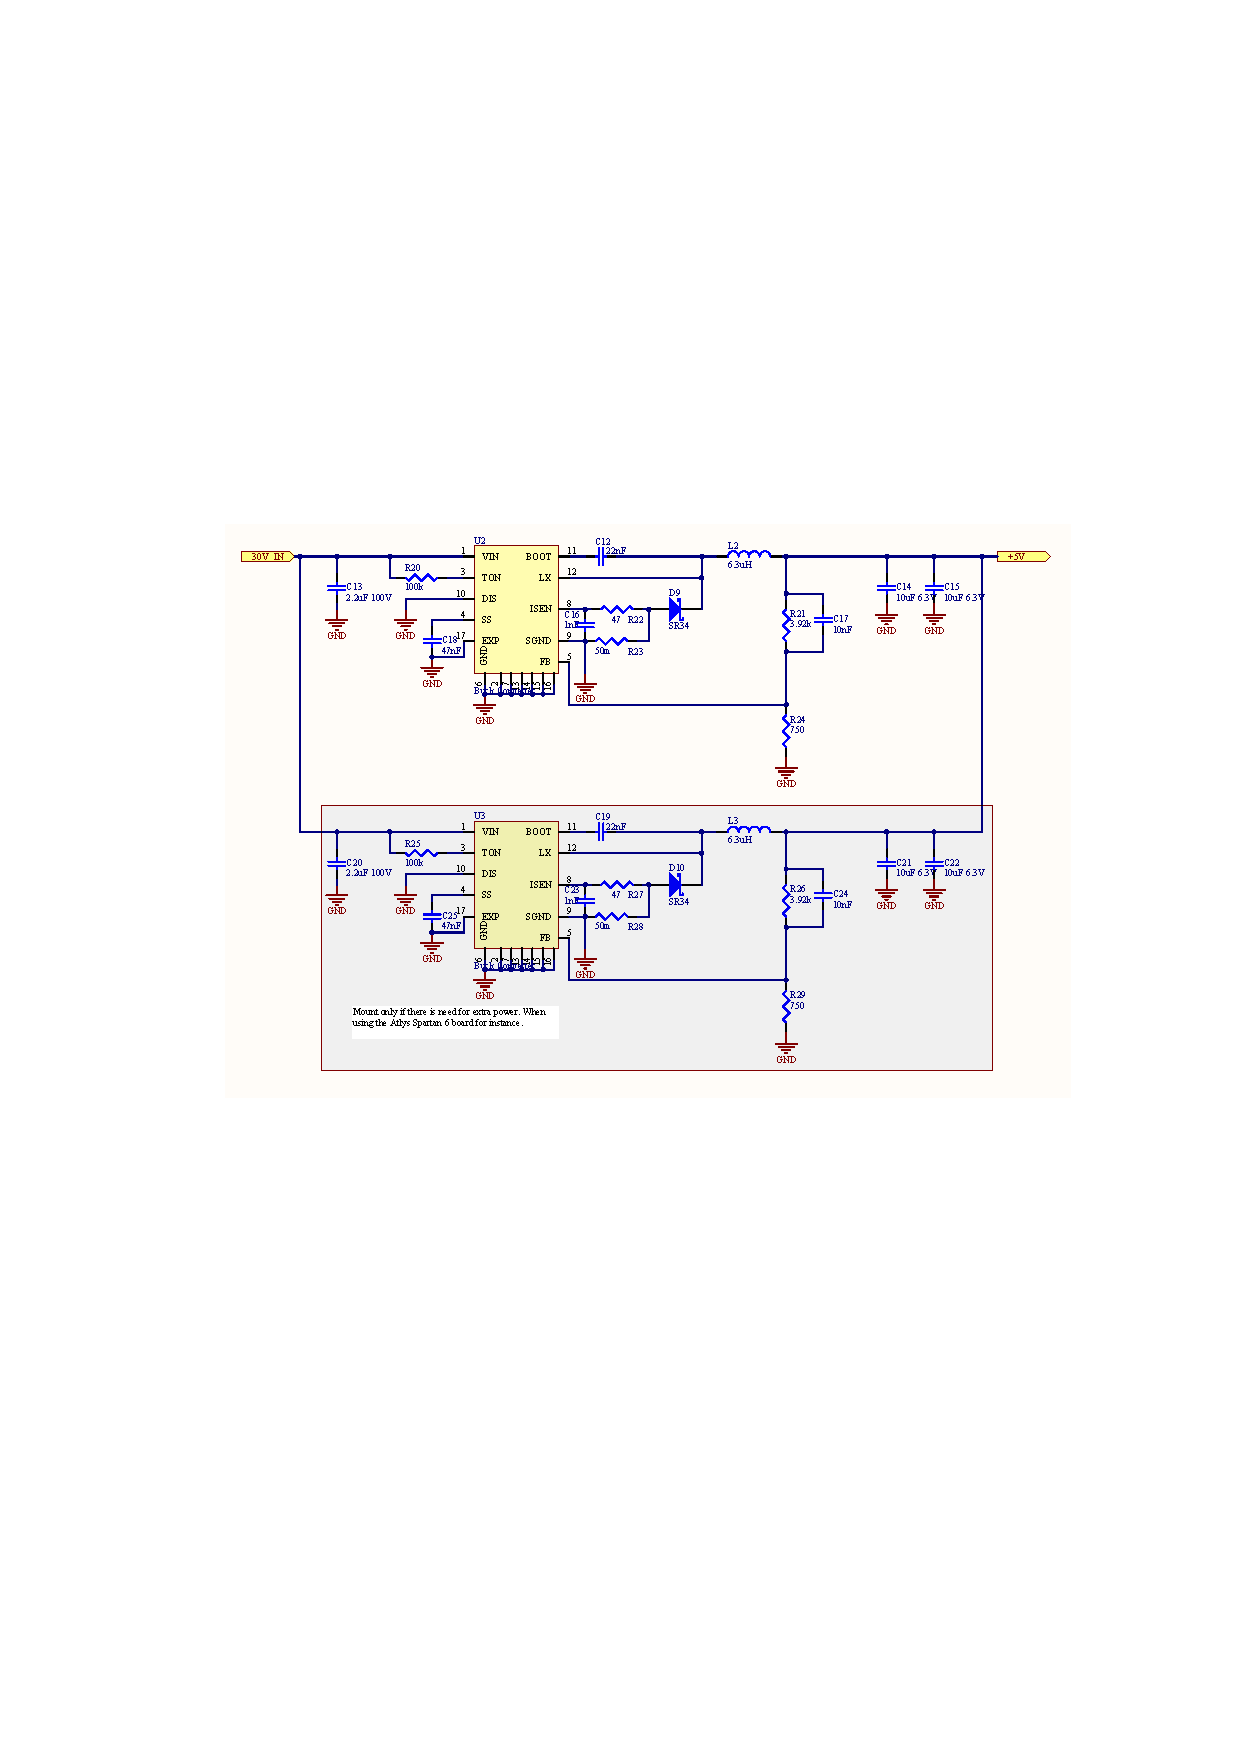
\includegraphics[width=0.9\textwidth,page=1,angle=0]{images/SIG60_v0_4}
		\caption{Power line circuit version 0.4}
	\end{centering}
\end{figure}

\begin{figure}[H]
	\begin{centering}
		 \includegraphics[width=0.8\textwidth,page=2,angle=0]{images/SIG60_v0_4}
		\caption{Power supply. 2 x 5 volt 3 ampere version 0.4.}
	\end{centering}
\end{figure}

\begin{figure}[H]
	\begin{centering}
		 \includegraphics[width=0.8\textwidth,page=3,angle=0]{images/SIG60_v0_4}
		\caption{PCB layout of the power line circuit and the 5 volt power supply version 0.4.}
	\end{centering}
\end{figure}

\todo[inline]{Insert photo of soldered PLC module}

\subsection{Daemon}
\subsubsection{Section Contents}
\begin{itemize}
	\item Overview
	\item Make daemon to run on uClinux
	\item The rc file (startup file)
	\begin{itemize}
		\item Configure network
		\item Start daemon as background process
	\end{itemize}
	\item Further implementations
	\imte Documentation (Generated on Doxygen)
\end{itemize}

\subsubsection{Overview}
\subsubsection{Make daemon to run on uClinux}
\subsubsection{The rc file (startup file)}
\subsubsubsection{Configure Network}
\subsubsubsection{Start daemon as background process}
\subsubsection{Further implementations}
\subsubsection{Documentation (Generated on Doxygen)}



\subsection{Power switch - Dennis}
The power switch is the part of the hub that traffics the energy from and to its connected modules, such as: wind-turbine, photovoltaics, hydrogen-cell, battery-storage, load modules and similar. Inspiration to the creation of the power switch has been found at: Powerhub Systems \footnote{\url{http://www.pwrhub.com/}} (routing system) and TORC \footnote{\url{http://www.torcrobotics.com/products/powerhub}} (implementation and control of the hub).
\subsubsection{Block diagram}
The switch is divided in 10 similar blocks (one for each module). Figure \ref{fig:ps_block_v0_1} shows an two modules connected to the power line. The content inside the dotted line block is an abstract description of the power switch. For simplicity two diodes has been used, to control the routing direction.
\begin{figure}[H]
	\begin{centering}
		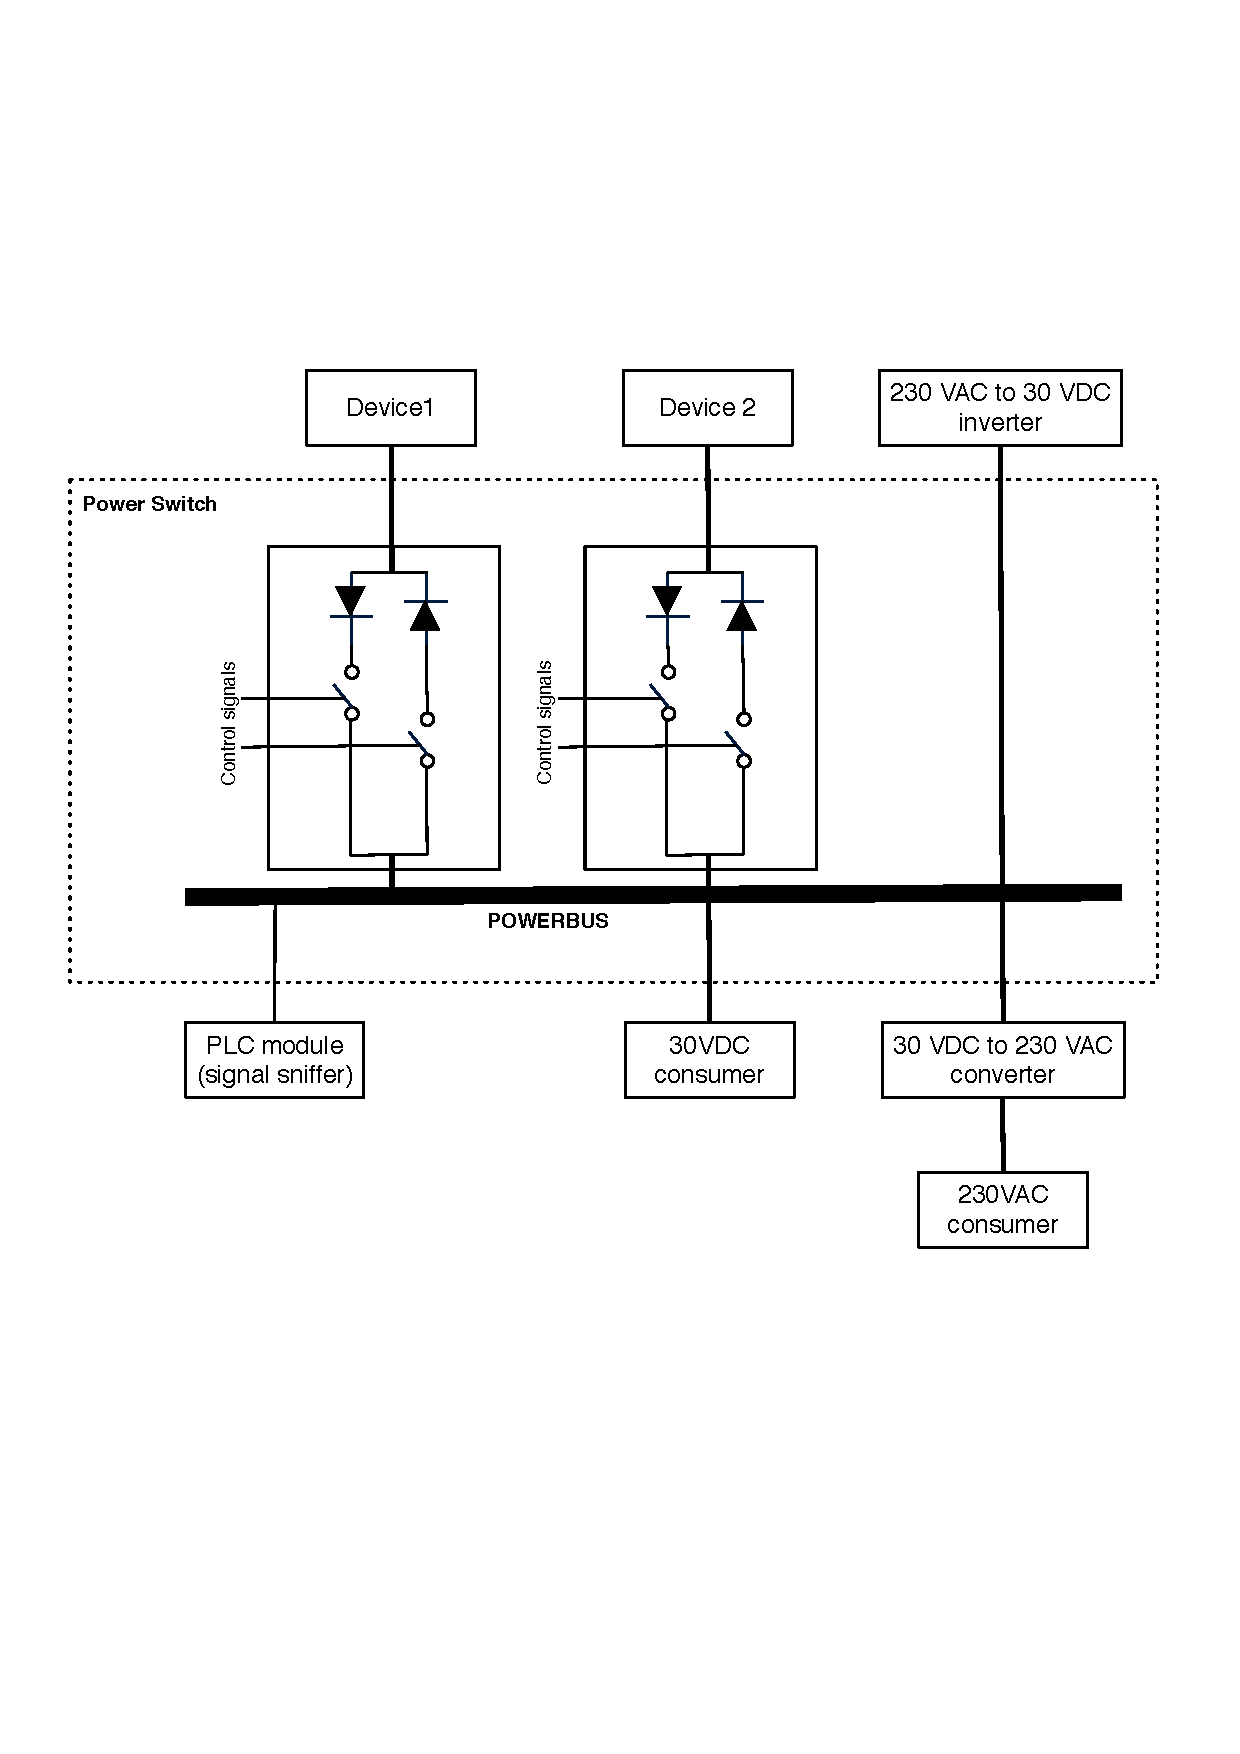
\includegraphics[width=0.8\textwidth,page=1,angle=0]{images/power_switch_block_diagram_v0_1}
		\caption{Block diagram of the Power Switch v0.1}
		\label{fig:ps_block_v0_1}
	\end{centering}
\end{figure}
The inverter is used to get energy to start up the system. Energy is also taken from the inverter if the energy-producing- and energy-storing modules cannot deliver enough. 
\p Notice that noise from switching devices on and of shall be minimized to not bother the power line module and in worst case manipulate with the data-packages. 
\p Two signals from the processor will be needed to control each of the switch blocks, however a control section might be added to the switch to decrease the number of pins needed to control all 10 blocks + consumers. 
\p Current measuring for the consuming devices and the inverter will be implemented in the switch, to keep track of how green the system is and if the producers are producing anything.  
\subsubsection{Diagram and components}
Some alternative components to diodes have been found, in order to control the current direction and have as little power loss as possible in the switch. 
\textbf{Component suggestions:}
\begin{itemize}
	\item Control device for MOSFETS, LTC4357\footnote{\url{http://www.linear.com/product/LTC4357}} from Linear Technology.
	\item Demo board for LTC4357\footnote{\url{http://cds.linear.com/docs/Demo\%20Board\%20Manual/dc1203A.pdf}}.
	\item Power Mosfets IRFP4468PbF\footnote{\url{http://pdf1.alldatasheet.com/datasheet-pdf/view/234175/IRF/IRFP4468PBF.html}} with low on resistance and maximum drain current of approximately 200Amps. \textit{Rds}
	\item If needed, dual power rectifiers MBR60H100CT\footnote{\url{http://pdf1.alldatasheet.com/datasheet-pdf/view/172142/ONSEMI/MBR60H100CT.html}}, with max. voltage on 100V and max. current on 60 Amps.
\end{itemize}
An initial diagram drawing have been made with two LTC4357 devices. The diagram shows the possible implementation of a single switch block.

\todo[inline]{draw diagram with 2 x LTC4357 + FETS (single block)}

\subsection{Module design}


